% cd ..\..\Users\NikitaSkybytskyi\Desktop\c3s2\numerical-analysis\lab\lab-7\tex
% cls && pdflatex report.tex && cls && pdflatex report.tex && cls && pdflatex report.tex && start report.pdf
\documentclass[12pt, a4paper]{article}
\usepackage[T2A]{fontenc}
\usepackage[utf8]{inputenc}
\usepackage[english,ukrainian]{babel}
\usepackage{amsmath, amssymb}
\usepackage{verbatim}

\usepackage[top = 2 cm, left = 1 cm, right = 1 cm, bottom = 2 cm]{geometry}

\usepackage{float, graphicx}
\usepackage{amsthm}
\newtheorem{lemma}{Лема}
\newtheorem*{lemma*}{Лема}
\newtheorem{theorem}{Теорема}
\newtheorem*{theorem*}{Теорема}
\newtheorem{definition}{Визначення}
\newtheorem*{definition*}{Визначення}
\theoremstyle{definition}
\newtheorem{remark}{Зауваження}
\newtheorem*{remark*}{Зауваження}
\newtheorem{example}{Приклад}
\newtheorem*{example*}{Приклад}
\newtheorem{problem}{Задача}
\newtheorem*{problem*}{Задача}
\newtheorem{solution}{Розв'язок}
\newtheorem*{solution*}{Розв'язок}
\newtheorem{corollary}{Наслідок}
\newtheorem*{corollary*}{Наслідок}

\newcommand{\NN}{\mathbb{N}}
\newcommand{\RR}{\mathbb{R}}
\newcommand{\CC}{\mathbb{C}}
\newcommand{\HH}{\mathcal{H}}
\newcommand{\Min}{\displaystyle\min\limits}
\newcommand{\Max}{\displaystyle\max\limits}
\newcommand{\Sup}{\displaystyle\sup\limits}
\newcommand{\Sum}{\displaystyle\sum\limits}
\newcommand{\Prod}{\displaystyle\prod\limits}
\newcommand{\Int}{\displaystyle\int\limits}
\newcommand{\Iint}{\displaystyle\iint\limits}
\newcommand{\Lim}{\displaystyle\lim\limits}

\newcommand*\diff{\mathop{}\!\mathrm{d}}

\renewcommand{\bf}[1]{\textbf{#1}}
\renewcommand{\epsilon}{\varepsilon}
\renewcommand{\phi}{\varphi}

\DeclareMathOperator{\signum}{sign}
\DeclareMathOperator{\diam}{diam}
\DeclareMathOperator{\rang}{rang}
\DeclareMathOperator{\const}{const}
\DeclareMathOperator{\cond}{cond}
\DeclareMathOperator{\diagonal}{diag}

\numberwithin{equation}{section}

\setlength\parindent{0pt}
\allowdisplaybreaks

\newcommand{\cover}[2]{
\begin{center}
\hfill \break
	Міністерство освіти та науки України \\
	Київський національний університет імені Тараса Шевченка \\ 
	Факультет комп'ютерних наук та кібернетики \\
	Кафедра обчислювальної математики
\end{center}

\vfill 

\begin{center}
	\large{
		Звіт до лабораторної роботи №{#1} на тему: \\ 
		``{#2}''
	}
\end{center}

\vfill 

\begin{flushright}
	Виконав студент групи ОМ-3 \\
	Скибицький Нікіта
\end{flushright}

\vfill 

\begin{center}
    Київ, 2018 
\end{center}

\thispagestyle{empty} 
\newpage
}

\begin{document}

\cover{7}{Чисельне інтегрування \\ диференційних рівнянь}

\tableofcontents

\section{Постановка задачі}

Автомобіль маси $M$, який підтримується прижуною з демпфером, переміщується з постійною горизонтальною швидкістю. В момент часу $t = 0$ центр тяжіння автомобіля знаходиться на відстані $h_0$ від землі, і при цьому вертикальна швидкість відсутня. Надалі вертикальний зсув дороги від основного рівня описується функцією $x_0(t)$. \medskip

Припустимо, що пружина лінійна, з коефіцієнтом пружності $k$, а коефіцієнт демпфірування $r$ є нелінійною функцією відносно швидкості двох кінці демфера:
\begin{equation}
	\label{eq:r-def}
	r = r_0 \cdot \Big( 1 + c \cdot \big| \dot x - \dot x_0 \big| \Big).
\end{equation}

Легко показати, що зсув $x(t)$ центру тяжіння автомобіля є розв'язком звичайного диференціального рівняння другого порядку
\begin{equation}
	\label{eq:x-diff-eq}
	\ddot x = - \frac{1}{M} \cdot \Big( k \cdot \big(x - x_0\big) + r \cdot \big(\dot x - \dot x_0\big) \Big)
\end{equation}
з початковими умовами 
	\begin{equation}
	x(0) = \dot x(0) = 0.
\end{equation}

Обчислити $x(t)$ на проміжку $0 \le t \le t_{\text{max}}$ для контуру дороги, який описується функцією
\begin{equation}
	x_0(t) = A \cdot (1 - \cos (\omega t)),
\end{equation}
де $2 A$ --- максимальний зсув основного рівня. \medskip

Зауважимо, що для лінійного випадку ($c = 0$) докритичному, критичному, і позакритичному демпфіруванню відповідають значення коефіцієнта
\begin{equation}
	\xi = \frac{r}{2 \sqrt{k M}}
\end{equation}
менший, рівний, і більший одиниці відповідно. \medskip

Програма повинна виводити значення: $t$, $x_0(t)$, $x(t)$, $\dot x(t)$, $\xi(t)$. \medskip

Параметри задачі:
\begin{table}[H]
	\centering
	\begin{tabular}{|c|c|c|c|c|c|c|}
		\hline
		$M$ & $A$ & $\omega$ & $k$ & $t_{\text{max}}$ & $r_0$ & $c$ \\ \hline
		$10$ & $2$ & $7$ & $640$ & $5$ & $160$ & $1$ \\ \hline
	\end{tabular}
\end{table}

% \newpage

\section{Аналітичні маніпуляції}

\subsection{Попередня обробка моделі}

Позначимо $y = \dot x$, тоді $\dot y = \ddot x$ і маємо наступну систему:
\begin{system}
	\dot x &= y = f(t, x, y), \\
	\dot y &= - \dfrac{1}{M} \cdot \Big( k \cdot \big(x - x_0\big) + r \cdot \big(y - \dot x_0\big) \Big) = g(t, x, y).
\end{system}

Також зауважимо, що ми використовуємо функцію $\dot x_0(t)$, тому наведемо тут її явний вигляд:
\begin{equation}
	\dot x_0(t) = A \cdot \omega \cdot \sin(\omega t).
\end{equation}

\subsection{Метод Рунге-Кутти}

Для моделювання будемо використовувати явний метод Рунге-Кутти четвертого порядку для системи $2 \times 2$. \medskip

Спочатку обчислюються наступні коефіцієнти:
\begin{equation}
	\begin{aligned}
		k_1 &= h \cdot f(t, x, y), \\
		q_1 &= h \cdot g(t, x, y), \\
		k_2 &= h \cdot f(t + h / 2, x + k_1 / 2, y + q_1 / 2), \\
		q_2 &= h \cdot g(t + h / 2, x + k_1 / 2, y + q_1 / 2), \\
		k_3 &= h \cdot f(t + h / 2, x + k_2 / 2, y + q_2 / 2), \\
		q_3 &= h \cdot g(t + h / 2, x + k_2 / 2, y + q_2 / 2), \\
		k_4 &= h \cdot f(t + h, x + k_3, y + q_3), \\
		q_4 &= h \cdot g(t + h, x + k_3, y + q_3),
	\end{aligned}
\end{equation}

А потім виконуються наступні кроки за відповідними координатами:
\begin{equation}
	\begin{aligned}
        t &\pluseqq h, \\
       	x &\pluseqq (k_1 + 2 k_2 + 2 k_3 + k_4) / 6, \\
        y &\pluseqq (q_1 + 2 q_2 + 2 q_3 + q_4) / 6.
	\end{aligned}
\end{equation}

\section{Чисельне моделювання}

\subsection{Графіки}

Було отримано наступні графіки:

\subsubsection{Висота центру мас і вертикальна швидкість авто}
\begin{figure}[H]
	\centering
	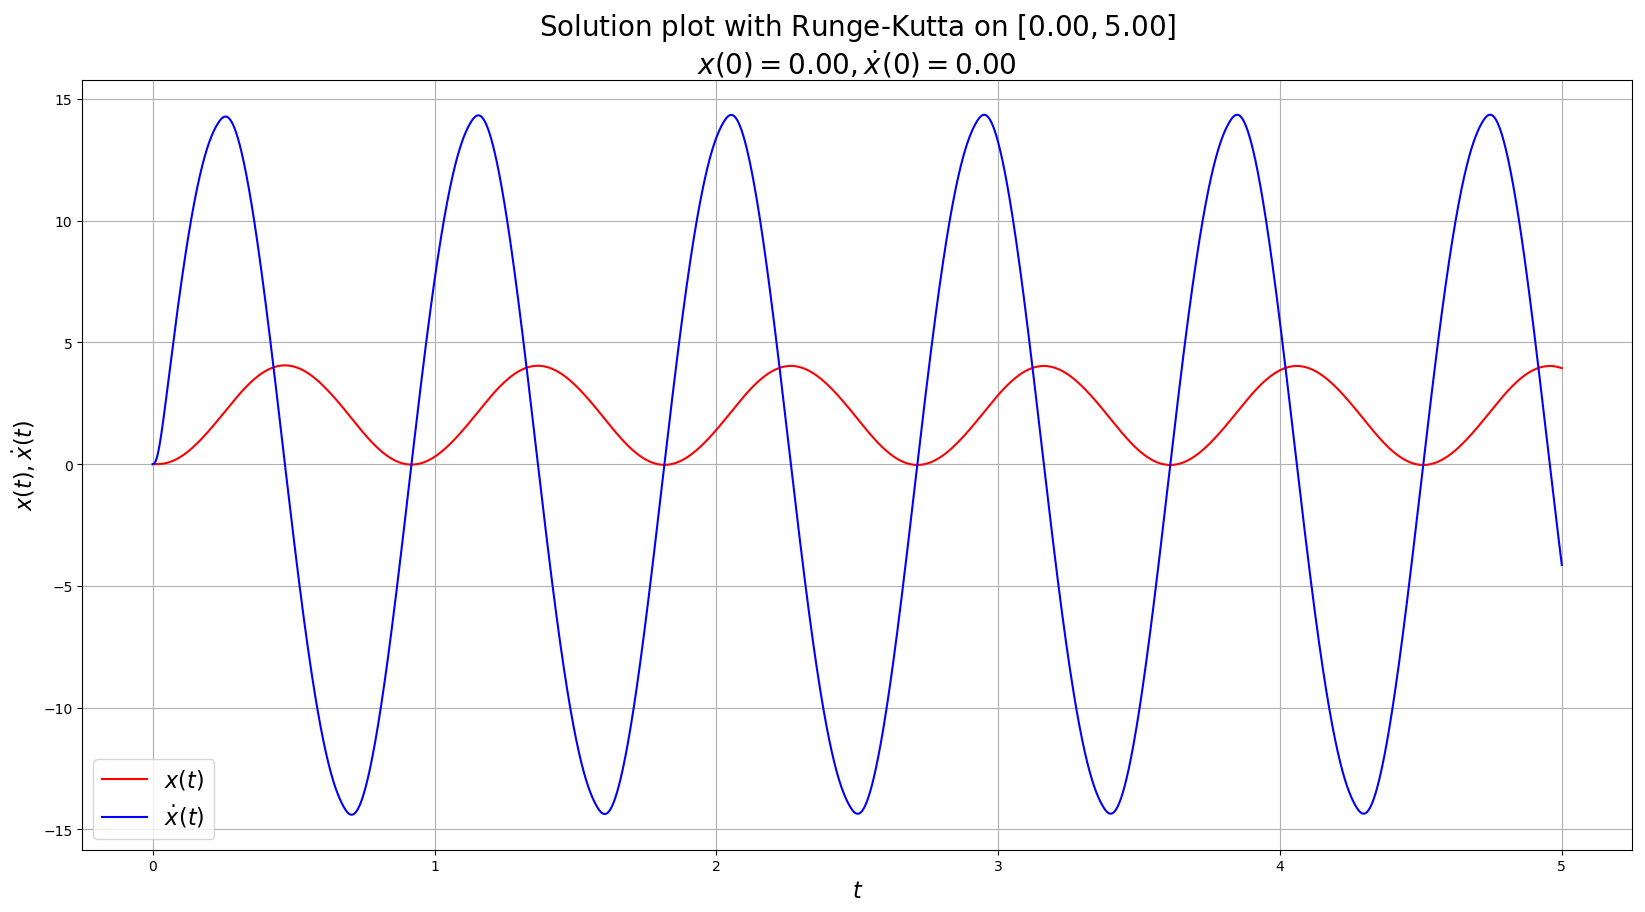
\includegraphics[width=\textwidth]{1.png}
\end{figure}

\subsubsection{Висота дороги і центру мас автомобіля}
\begin{figure}[H]
	\centering
	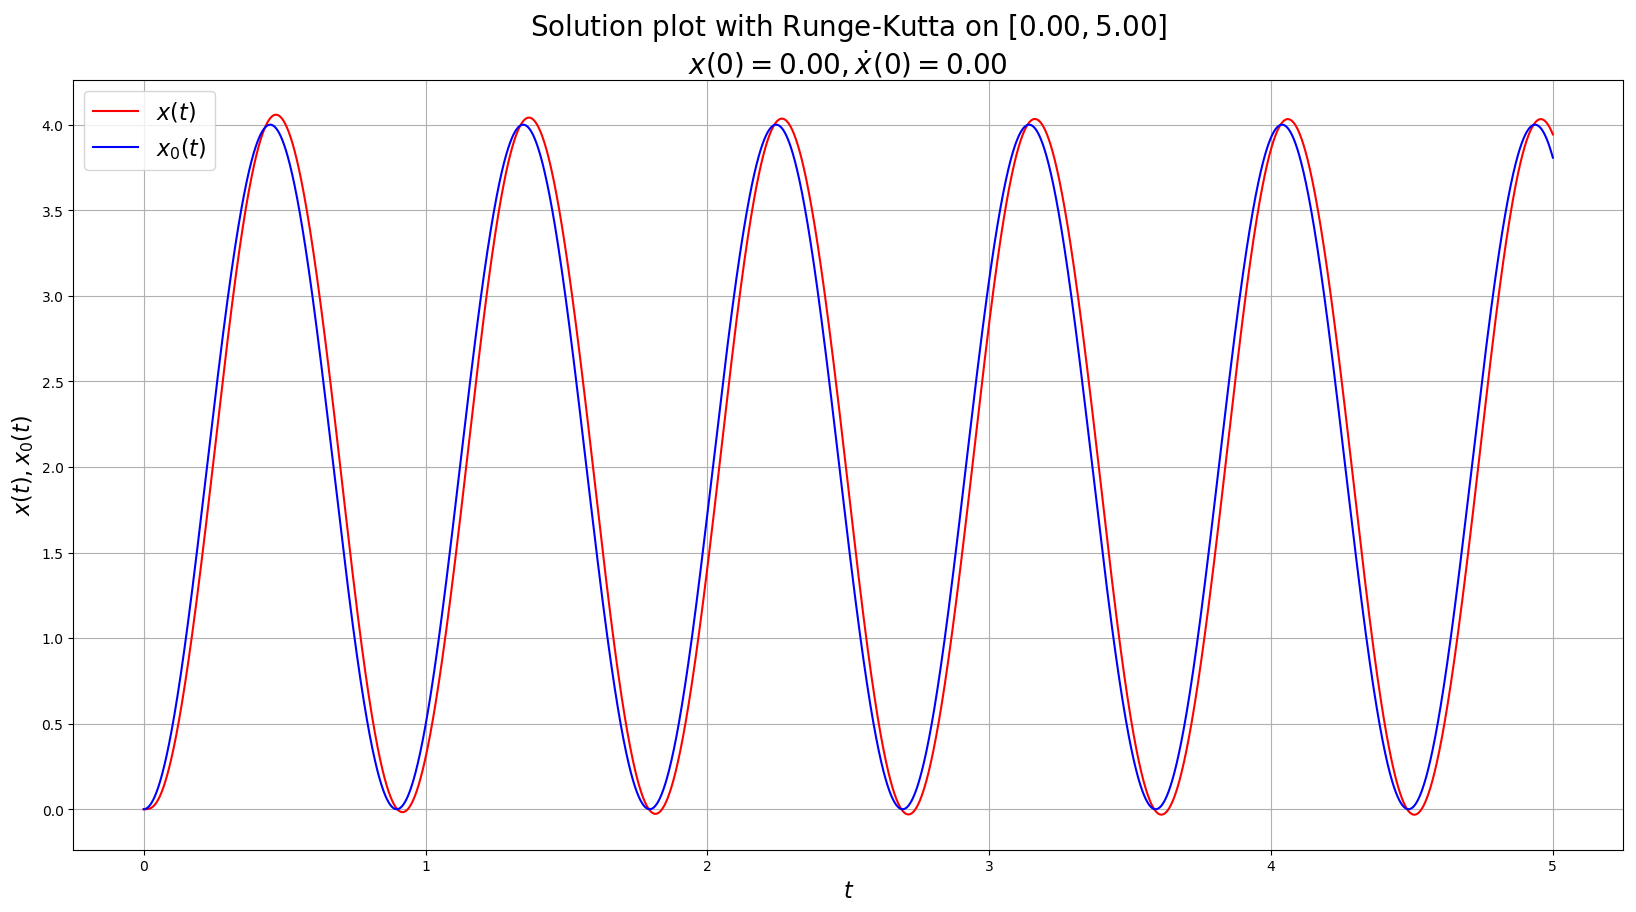
\includegraphics[width=\textwidth]{2.png}
\end{figure}

Зауважимо, що висота центру мас авто нібито буває ``нижче'' ніж рівень дороги, бо тут не враховується висота $h_0$, а варто було б.

\subsubsection{Внесок демпфера у вертикальний рух}
\begin{figure}[H]
	\centering
	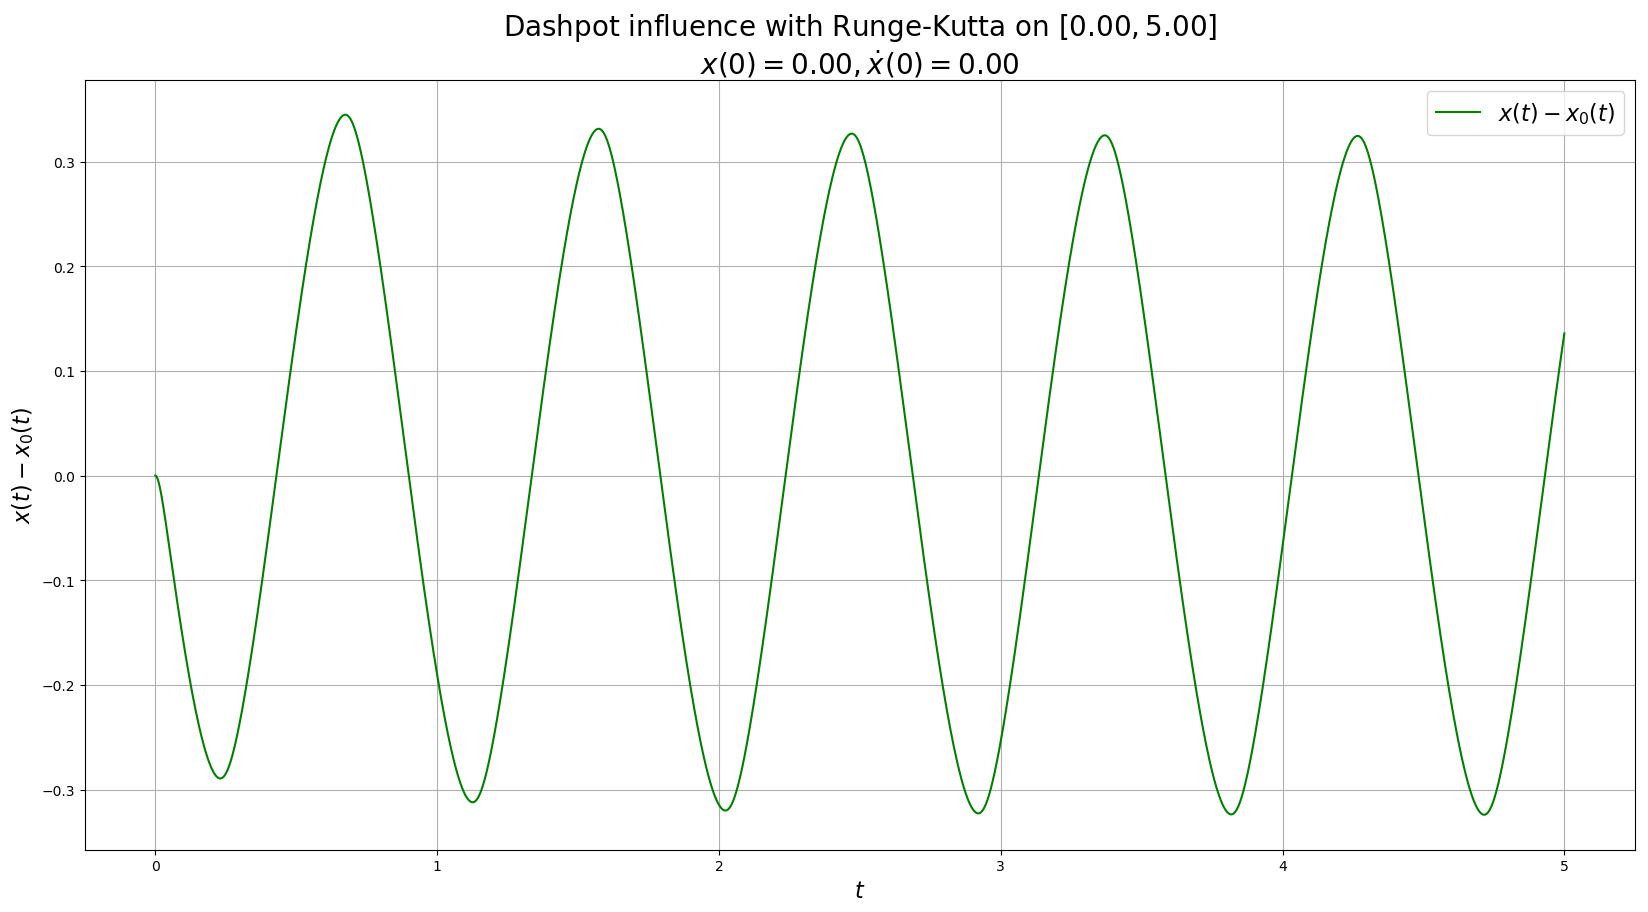
\includegraphics[width=\textwidth]{3.png}
\end{figure}

\subsubsection{Критичність навантаження на демпфер}
\begin{figure}[H]
	\centering
	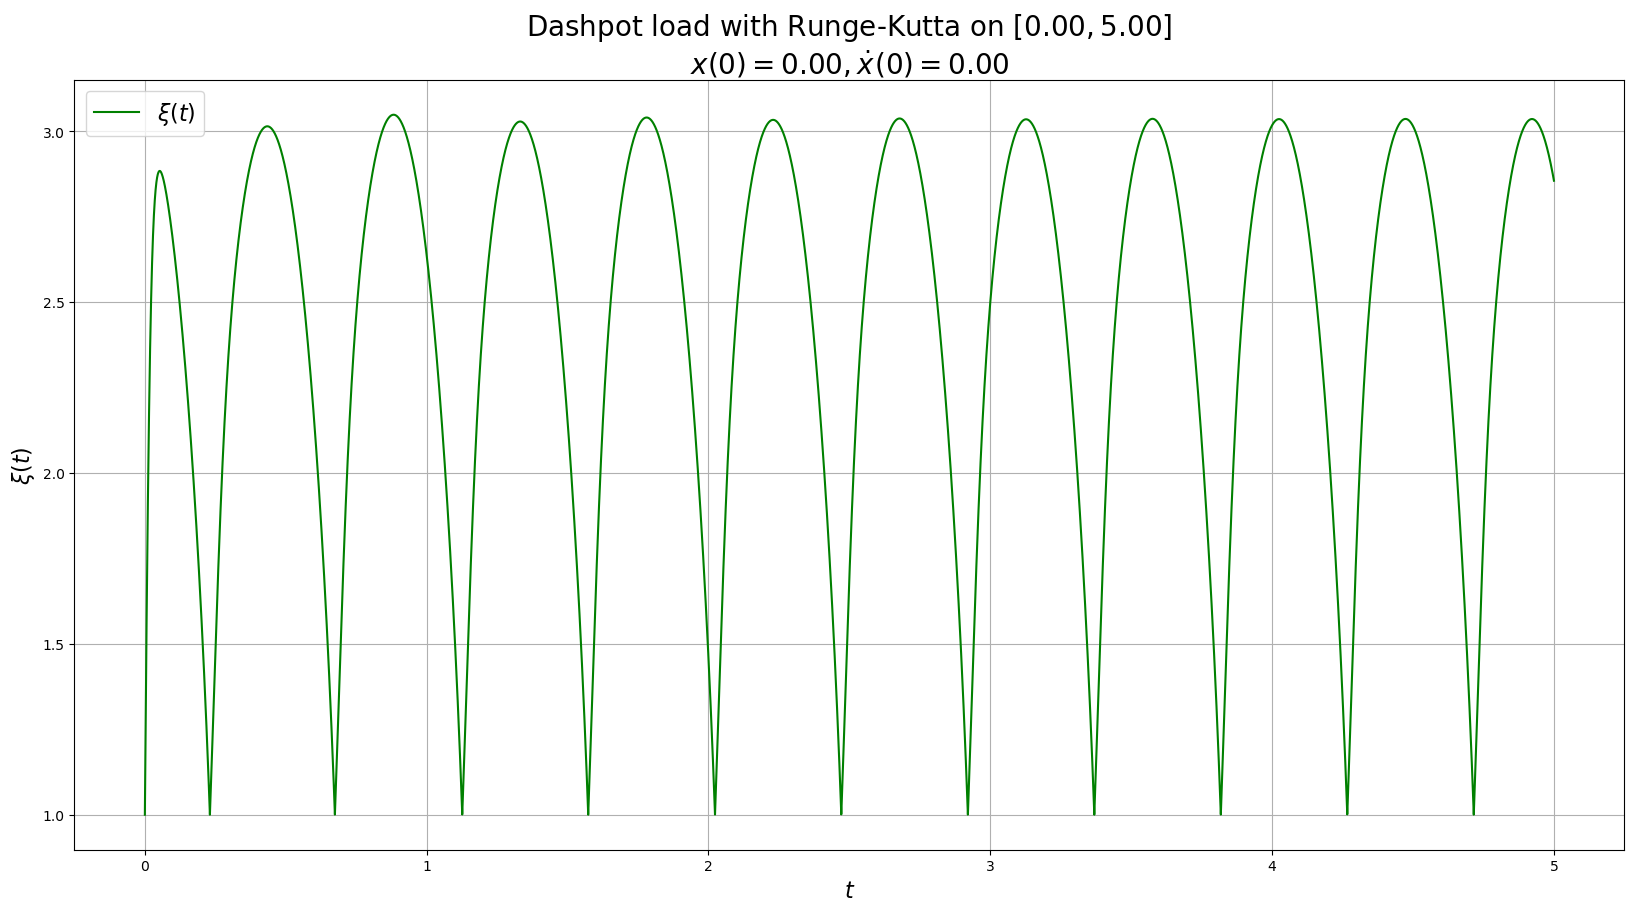
\includegraphics[width=\textwidth]{4.png}
\end{figure}

\subsection{Код}

\subsubsection{Модель демпфера}

Для моделювання демпфера було написано наступний клас:
\inputminted[firstline=5, lastline=33]{python}{../py/dashpot.py}

Як бачимо, він зберігає в собі внутрішні незмінні параметри демпфера, а також надає функціональність для обчислення коефіцієнту демпфірування і значененя рівня критичності демпфірування. Обидва згадані методи потребують також відомостей про ``зовнішній світ''.

\subsubsection{Модель машини}

Для моделювання машини було написано наступний клас:
\inputminted[firstline=5, lastline=35]{python}{../py/car.py}

Як бачимо, він зберігає в собі внутрішні незмінні параметри машини (включаючи положення машини, і параметри демпфера цієї машини), а також надає функціональність для обчислення коефіцієнту демпфірування і значененя рівня критичності демпфірування. Обидва згадані методи потребують також відомостей про ``зовнішній світ''.

\subsubsection{Модель дороги}

Для моделювання дороги було написано наступний клас:
\inputminted[firstline=5, lastline=26]{python}{../py/road.py}

Як бачимо, він зберігає в собі внутрішні незмінні параметри дороги, а також надає функціональність для обчислення положення дороги під машиною у певний момент часу. 

\subsubsection{Модель сцени (фізичного світу)}

\textit{Сценою} (eng. \textit{stage}) у програмуванні прийнято називати клас, що містить і контролює життя усіх об'єктів які моделюються. \medskip

Для моделювання сцени було написано наступний клас:
\inputminted[firstline=7, lastline=74]{python}{../py/stage.py}

Як бачимо, він містить метод \verb|move| який і відповідає за моделювання поведінки усіх об'єктів що перебувають на сцені.

\subsubsection{Програма-драйвер}

Окремо від вищезгаданих класів було написано програму-драйвер:
\inputminted[firstline=9, lastline=85]{python}{../py/main.py}

Як бачимо, вона не містить жодної складної логіки (у чому і була суть допоміжних класів), тобто зі сторони клієнту робота з реалізованою класами функціональністю дуже проста. \medskip

Єдиною хоча б трохи цікавою особливістю коду, яка вспливає тілкьи у програмі-драйвері є можливість друкувати у людському форматі стан сцени (а також машини, демпфера, і дороги), приблизно у такому форматі:
\begin{minted}{python}
Stage(t=0, 
	car=Car(
		x=0, dot_x=0, m=10, 
		dashpot=Dashpot(k=640, r_0=160, c=1)
	), 
	road=Road(a=2, omega=7)
)
\end{minted}

або
\begin{minted}{python}
Stage(t=1.2345000, 
	car=Car(
		x=3.2203857, dot_x=11.6096103, m=10, 
		dashpot=Dashpot(k=640, r_0=160, c=1)
	), 
	road=Road(a=2, omega=7)
)
\end{minted}

\end{document}
